\labeledsection{Inductive Logic Programming}{sec:inductive_logic}
\titledbox{Motivation}{
\begin{itemize}
    \item Previously, we talked about learning from examples (\linkterm{inductive learning}{supervised_learning})
    \item Main idea was $\leadsto$ constructing a \linkterm{function}{function} with the input-output behavior observed in the data
    \item The main method was searching for suitable \linkterm{hypothesis}{supervised_learning} in a \linkterm{hypothesis space}{supervised_learning}
    \item Every learning task begins from zero except we choose the \linkterm{hypothesis space}{supervised_learning}
\end{itemize}
}

\problembox{
We have to forget anything before we can learn something new
}

\ideabox{
Utilize prior knowledge about the world
}

\questionbox{How can we do that?}

\titledbox{Remember}{
\linkterm{examples}{supervised_learning} are composed of descriptions of the input sample and classifications
}

\ideabox{
Represent \linkterm{examples}{supervised_learning} and \linkterm{hypotheses}{supervised_learning} as logical formulae
}

\Example{
We can make \linkterm{attribute-based representation}{attribute_based_representations} using the language of First-Order Logic (\linkterm{$\text{PL}^1$}{pl1}). We can use \linkterm{predicate constants}{fol_sig_pl1} for Boolean attributes and classifications and \linkterm{function constants}{fol_sig_pl1} for other attributes.
}{}

\noindent\makebox[\textwidth]{%
\rule{0.25\textwidth}{0.4pt}\hfill
\textbf{Excursion : Recall - First-Order Logic}\hfill
\rule{0.25\textwidth}{0.4pt}%
}

\anondefinition{
\defemph{First-Order (Predicate) Logic} $\text{PL}^1$ is a \linkterm{formal system}{formal_system} extensively used in mathematics, philosophy, linguistics, and computer science. It combines \linkterm{$\text{PL}^0$}{def:pl0_as_ls} with the ability to quantify over \linkterm{individuals}{fol_sig}
}{pl1}

\anondefinition{
A \defemph{First-Order Signature} is a tuple $\Sigma := \tuple{\Sigma_1, \linkterm{\Sigma_0}{wff0_def}}$ where $\Sigma_1 := \Sigma^f \cup \Sigma^p \cup \Sigma^{sk}$:
\begin{itemize}
\item $\Sigma^f := \bigcup_{k \in \mathbb{N}} \Sigma_k^f$ of \textbf{function constants} (or \textbf{terms}), where members of $\Sigma_k^f$ denote the $k$-ary \linkterm{functions}{function} on \textbf{individuals}
\item $\Sigma^p := \bigcup_{k \in \mathbb{N}} \Sigma_k^p$ of \textbf{predicate constants}, where member of $\Sigma_k^p$ denote $k$-ary \linkterm{relations}{relation} among individuals
\item $\Sigma^{sk} := \bigcup_{k \in \mathbb{N}} \Sigma_k^{sk}$ of \textbf{Skolem constants} that act as witness constructors
\item All are \linkterm{pairwise disjoint}{pairwise_disjoint}, \linkterm{countable}{countable} \linkterm{sets}{def:set} of symbols for each $k \in \mathbb{N}$.
\end{itemize}
We also assume a \linkterm{set}{def:set} of \textbf{individual variables} $V_{\iota} := \set{X,Y,Z,\cdots}$ which we can quantify over them.
}{fol_sig_pl1}


\definition{\linkterm{$\text{PL}^1$}{pl1} Terms}{
The \linkterm{set}{def:set} $\text{wff}_{\iota}(\Sigma_1, V_{\iota})$ of \textbf{well-formed terms} over the signature $\Sigma_1$ and variables \linkterm{$V_{\iota}$}{fol_sig_pl1} is defined by the following \linkterm{grammar}{phrase_structure_grammar}:
\begin{align*}
f^k \quad &\in \quad \Sigma_k^f \cup \Sigma_k^{sk} \\
X \quad &\in \quad \linkterm{V_{\iota}}{fol_sig_pl1} \\ 
t \quad &::= \quad X \mid f^k(t_1, \cdots, t_k)
\end{align*}
}{terms_pl1}

\definition{\linkterm{$\text{PL}^1$}{pl1} Propositions}{
The \linkterm{set}{def:set} $\text{wff}_{\circ}(\Sigma_1, V_{\iota})$ of \textbf{well-formed formulae} over the signature $\Sigma_1$ and variables \linkterm{$V_{\iota}$}{fol_sig_pl1} is defined by the following \linkterm{grammar}{phrase_structure_grammar}:
\begin{align*}
p^k \quad &\in \quad \Sigma_k^p \\
t_i \quad &\in \quad \text{wff}_{\iota}(\Sigma_1, \linkterm{V_{\iota}}{fol_sig_pl1}) \\ 
X \quad &\in \quad \linkterm{V_{\iota}}{fol_sig_pl1} \\ 
A \quad &::= \quad p^k(t_1, \cdots, t_k) \mid \top \mid \neg A \mid A \land A \mid \forall X.A
\end{align*}
}{formulae_pl1}

\anondefinition{
The \textbf{universal quantifier} $\forall$ is a binding operator used to express $\forall X.A$, i.e. a \linkterm{formula}{formulae_pl1} $A$ holds for all possible values of an \linkterm{individual variable}{terms_pl1} $X \in$ \linkterm{$V_{\iota}$}{fol_sig_pl1}
}{forall}

\anondefinition{
The \textbf{existential quantifier} $\exists$ is a binding operator defined as an \textbf{abbreviation} for a negated universal statement: $\exists X.A :\equiv \neg (\forall X. \neg A)$. It allows us to express that at least one \linkterm{individual}{terms_pl1} satisfies the \linkterm{formula}{formulae_pl1} $A$.
}{exists}

\anondefinition{
A \linkterm{formula}{formulae} is called \textbf{atmoic} (or an \textbf{atom}) if it does not contain logical constants, otherwise, \textbf{complex}
}{atomic_formula}

\anondefinition{
Let $\mathcal{S} := \langle \mathcal{L}, \mathcal{M}, \vDash \rangle$ be a \linkterm{logical system}{logical_system}, $A \in \mathcal{L}$ a formula, $L$ a \textbf{label set}, and $\alpha \in L$ a \textbf{label}, then we call a \linkterm{pair}{cartesian_product} $\tuple{A, \alpha}$ a \textbf{labeled formula} and write it as $A^{\alpha}$. For a \linkterm{set}{def:set} $\Phi$ of \linkterm{propositions}{proposition} we use $\Phi^{\alpha} := \set{A^{\alpha} \mid A \in \Phi}$
}{labeled_formula}

\anondefinition{
Let $\mathcal{S} := \langle \mathcal{L}, \mathcal{M}, \vDash \rangle$ be a \linkterm{logical system}{logical_system}, $A \in \mathcal{L}$ is an \linkterm{atomic formula}{atomic_formula}, and $\alpha \in \set{T,F}$, then we call the \linkterm{labeled formula}{labeled_formula} $A^{\alpha}$ a \textbf{literal}.
}{literal}


\noindent\makebox[\textwidth]{%
\rule{0.3\textwidth}{0.4pt}\hfill
\textbf{End of Excursion}\hfill
\rule{0.3\textwidth}{0.4pt}%
}

\anondefinition{
\defemph{Logic-based inductive learning} tries to learn a \linkterm{hypothesis}{supervised_learning} $h$ that explains the \linkterm{classifications}{classifcation_regression} of the \linkterm{examples}{supervised_learning} given their \defemph{description}, i.e. $h, \mathcal{D} \sat \mathcal{C}$ (the \defemph{explanation constraint}), where:
\begin{itemize}
    \item $\mathcal{D}$ is the conjunction of the \defemph{descriptions}, and
    \item $\mathcal{C}$ is the conjunction of their \linkterm{classifications}{classifcation_regression}
\end{itemize}
}{logic_based_inductive_learning}

\commandnote{
The idea is that we solve the \linkterm{explanation constraint}{logic_based_inductive_learning} for $h$ where $h$ ranges over some \linkterm{hypothesis space}{supervised_learning}
}

\Example{
Remember \Exampleref{restaurant_example}:

\begin{tabular}{c||c|c|c|c|c|c|c|c|c|c||c}
\hline
 & \multicolumn{10}{c||}{\textbf{Attributes}} & \textbf{Target} \\ \cline{2-11}
\textbf{Example} & \textit{Alt} & \textit{Bar} & \textit{Fri} & \textit{Hun} & \textit{Pat} & \textit{Price} & \textit{Rain} & \textit{Res} & \textit{Type} & \textit{Est} & \textit{WillWait} \\ \hline\hline
$X_1$  & T & F & F & T & Some & \$\$\$ & F & T & French  & 0--10  & T \\ 
$X_2$  & T & F & F & T & Full & \$    & F & F & Thai    & 30--60 & F \\ 
$X_3$  & F & T & F & F & Some & \$    & F & F & Burger  & 0--10  & T \\ 
$X_4$  & T & F & T & T & Full & \$    & F & F & Thai    & 10--30 & T \\ 
$X_5$  & T & F & T & F & Full & \$\$\$ & F & T & French  & $>$60  & F \\ 
$X_6$  & F & T & F & T & Some & \$\$   & T & T & Italian & 0--10  & T \\ 
$X_7$  & F & T & F & F & None & \$    & T & F & Burger  & 0--10  & F \\ 
$X_8$  & F & F & F & T & Some & \$\$   & T & T & Thai    & 0--10  & T \\ 
$X_9$  & F & T & F & T & Full & \$    & T & F & Burger  & $>$60  & F \\ 
$X_{10}$ & T & T & T & T & Full & \$\$\$ & F & T & Italian & 10--30 & F \\ 
$X_{11}$ & F & F & F & F & None & \$    & F & F & Thai    & 0--10  & F \\ 
$X_{12}$ & T & T & T & T & Full & \$    & F & F & Burger  & 30--60 & T \\ \hline
\end{tabular}

\linkterm{descriptions}{logic_based_inductive_learning} are conjunctions of \linkterm{literals}{literal} built up from
\begin{itemize}
    \item \linkterm{predicates}{fol_sig_pl1} \texttt{Alt}, \texttt{Bar}, \texttt{Fri/Sat}, \texttt{Hun}, \texttt{Rain}, \texttt{Res}
    \item Equations about the \linkterm{functions}{fol_sig_pl1} \texttt{Pat}, \texttt{Price}, \texttt{Type}, \texttt{Est}
\end{itemize}
For instance, the first \linkterm{example}{supervised_learning} $X_1$ can be described as:
\[
\text{Alt}(X_1) \land \neg \text{Bar}(X_1) \land \neg \text{Fri/Sat}(X_1) \land \text{Hun}(X_1) \land
\text{Pat}(X_1) = \text{Some} \land \cdots
\]
The \linkterm{classification}{classifcation_regression} is given by the goal \linkterm{predicate}{fol_sig_pl1} \texttt{WillWait}, in this case $\text{WillWait}(X_1)$ or $\neg \text{WillWait}(X_1)$
}{}


\Example{
Remember the induced \linkterm{DT}{decision_trees} from \Exampleref{ex:learned_dt}:
\begin{center}
    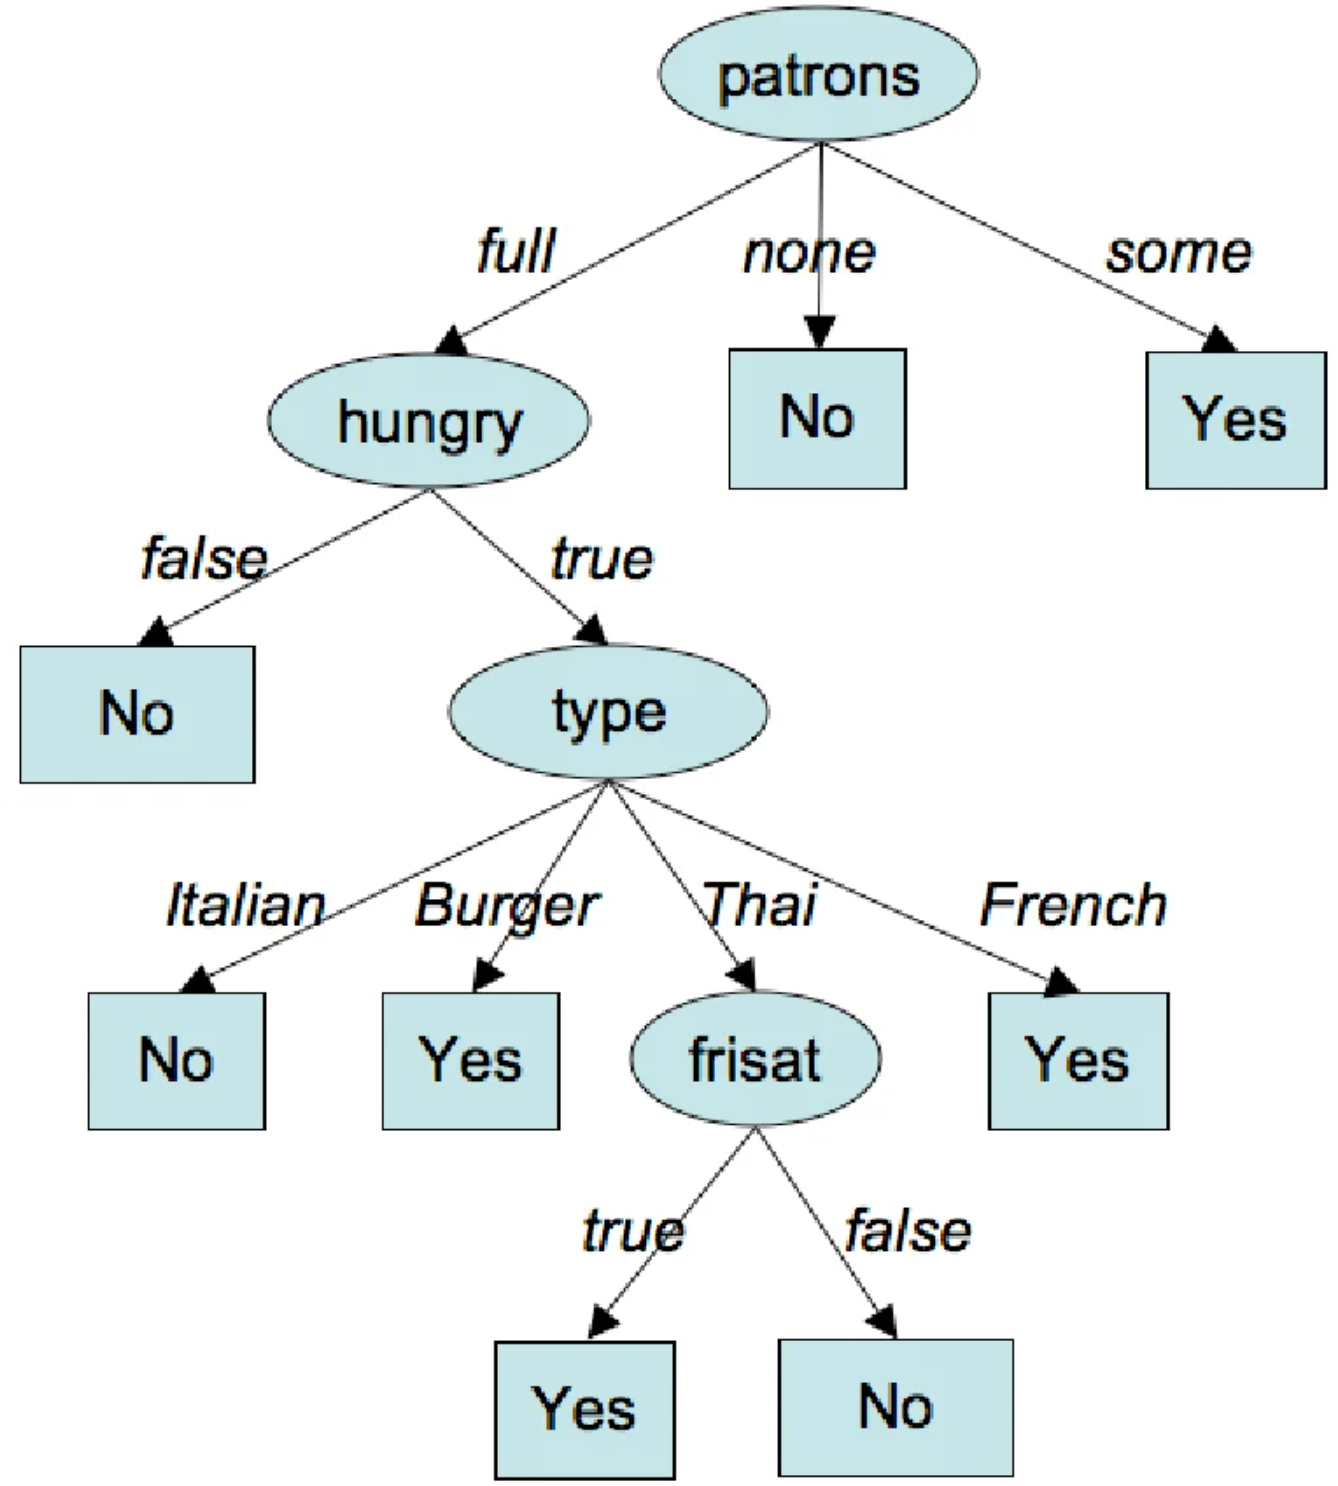
\includegraphics[width=0.3\linewidth]{images/restaurant_dtl.png}
\end{center}
This can be expressed as:
\begin{align*}
\forall r. \text{WillWait}(r) &\Leftrightarrow \text{Pat}(r, \text{Some}) \\ 
&\lor \text{Pat}(r, \text{Full}) \land \text{Hun}(r) \land \text{Type}(r, \text{French}) \\ 
&\lor \text{Pat}(r, \text{Full}) \land \text{Hun}(r) \land \text{Type}(r, \text{Thai}) \land \text{Fri/Sat}(r) \\ 
&\lor \text{Pat}(r, \text{Full}) \land \text{Hun}(r) \land \text{Type}(r, \text{Burger})
\end{align*}

\textbf{Method: }construct a disjunction of all the \linkterm{paths}{path_graph} from teh \linkterm{root}{tree} to the positive \linkterm{leaves}{tree} interpreted as conjunctions of the \linkterm{attributes}{attribute_based_representations} on the \linkterm{path}{path_graph}

\textbf{Note: }The equivalence takes care of positive and negative \linkterm{examples}{supervised_learning}
}{}

\observationbox{
We can represent unary \linkterm{function constants}{fol_sig_pl1} as binary \linkterm{predicate constants}{fol_sig_pl1} by shifting the output value into a second argument position, eliminating the need for the equality symbol ($=$):
\[
\text{Function}(x) = \text{value} \quad\leadsto\quad \text{Predicate}(x, \text{value})
\]
For example, $\text{Type}(X_1) = \text{French}$ becomes $\text{Type}(X_1, \text{French})$.
}

\titledbox{Machine Learning vs Humans}{
\begin{itemize}
    \item Standard machine learning algorithms starts from scratch. To learn a new concept, they require hundreds of thousands of examples because they have to figure out all the rules of the world from data alone.
    \item In contrast, humans can learn a general rule from a single example because we do not start from zero; we use what we already know about the world to fast-track our understanding.
\end{itemize}
}

\Example{\textbf{Caveman Zog}: 

If Zog sees someone put a fish on a stick over a fire and it tastes good, he doesn't need to try cooking a hundred different fish on a hundred different sticks to form a hypothesis. He instantly generalizes: “Food on a stick over fire cooks well.” He uses his prior understanding of fire, wood, and eating.
}{}

\Example{\textbf{The Brazilian}: 

If you meet one Brazilian and they speak Portuguese, you immediately assume most Brazilians speak Portuguese. You don't need a sample size of 10,000 citizens because your background knowledge already includes the concept of "national languages."
}{}

\Example{\textbf{Johanna and the Antibiotic}: 

Johanna knows nothing about the drug Proxadone, but she knows the doctor is an expert, an inflamed foot indicates a bacterial infection, and antibiotics kill bacteria. From observing one single prescription, she infers that Proxadone is effective against foot infections.
}{}

\problembox{
\linkterm{Supervised learning}{supervised_learning} cannot replicate this.

}

\questionbox{Why?}

\answerbox{
Standard algorithms fail here because they lack context. If you feed a standard algorithm a dataset with a single row containing $[\text{Patient\_ID}, \text{Inflamed\_Foot}, \text{Proxadone}] \Rightarrow [\text{Cured}]$, it cannot statistically justify generalizing this to all future patients. It sees it as an isolated statistical fluke or a correlation of size 1.
}

\solutionbox{
To bridge this gap, \linkterm{logic-based learning}{logic_based_inductive_learning} explicitely introduces \defemph{Background Knowledge} $\mathcal{B}$. Instead of searching for a \linkterm{hypothesis}{supervised_learning} $h$ based only on the \linkterm{descriptions}{logic_based_inductive_learning} $\mathcal{D}$ and \linkterm{classifications}{classifcation_regression} $\mathcal{C}$, the \linkterm{explanation constraint}{logic_based_inductive_learning} is upgraded to include what the system already knows.
\[
\mathcal{B} \land h \land \mathcal{D} \sat \mathcal{C}
\]
}


\titledbox{Cumulative Development}{
The ultimate goal is \defemph{cumulative learning}
\begin{itemize}
    \item We start with some prior knowledge
    \item We observe the world and learn a new rule/\linkterm{hypothesis}{supervised_learning} efficiently using that prior knowledge.
    \item This new \linkterm{hypothesis}{supervised_learning} is validated, becomes true, and is added back into our body of background knowledge $\mathcal{B}$
    \item For the next learning task, our $\mathcal{B}$ is now larger and richer, making the next round of learning even faster and more sophisticated
\end{itemize}
}

\anondefinition{
We call the body of knowledge accumulated by (a group of) \linkterm{agents}{def:agent} their \defemph{background knowledge}. It acts as \defemph{prior knowledge} in \linkterm{logic-based learning}{logic_based_inductive_learning} processes
}{bg_knowledge}

\begin{figure}[H]
    \centering
    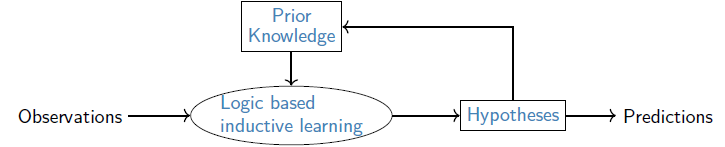
\includegraphics[width=0.5\linewidth]{images/logic_learning.png}  
\end{figure}

\anondefinition{
\defemph{Knowledge-based inductive learning (KBIL)} replaces the \linkterm{explanation constraint}{logic_based_inductive_learning} by the \defemph{KBIL constraint}:
\[
\mathcal{B} \land h \land \mathcal{D} \sat \mathcal{C}
\]
}{KBIL}

\centeredtitledbox{Remember \Defref{def:reasoning}}{
Deduction $\hat{=}$ knowledge extension
\Example{
\[
    \infer[D]{\text{wet\_street}}{\text{rains} \Rightarrow \text{wet\_street} \quad \text{rains}}
\]
}{}

Abduction $\hat{=}$ explanation
\Example{
\[
    \infer[A]{\text{rains}}{\text{rains} \Rightarrow \text{wet\_street} \quad \text{wet\_street}}
\]
}{}

Induction $\hat{=}$ learning general rules from \linkterm{examples}{supervised_learning}
\Example{
\[
    \infer[I]{\text{rains} \Rightarrow \text{wet\_street}}{\text{wet\_street} \quad \text{rains}}
\]
}{}
}

\anondefinition{
\defemph{Inductive Logic Programming (ILP)} is a \linkterm{logic-based inductive learning method}{logic_based_inductive_learning} that uses logic programming as a uniform representation for \linkterm{examples}{supervised_learning}, \linkterm{background knowledge}{bg_knowledge} and \linkterm{hypotheses}{supervised_learning}. Given an encoding of the known \linkterm{background knowledge}{bg_knowledge} and a \linkterm{set}{def:set} of \linkterm{examples}{supervised_learning} represented as logical knowledge base of facts, an \defemph{ILP} system will derive a hypothesized logic program which entails all the positive and none of the negative \linkterm{examples}{supervised_learning}
}{ILP}

\commandnote{
\linkterm{Prior knowledge}{bg_knowledge} plays two key roles:
\begin{itemize}
    \item The effective \linkterm{hypothesis space}{supervised_learning} is reduced to include only those theories that are consistent with what is already known
    \item \linkterm{Prior knowledge}{bg_knowledge} can be used to reduce the size of the \linkterm{hypothesis}{supervised_learning} explaining the observations $\leadsto$ smaller \linkterm{hypotheses}{supervised_learning} are easier to find
\end{itemize}
}

\observationbox{
\linkterm{ILP}{ILP} systems can formulate \linkterm{hypotheses}{supervised_learning} in \linkterm{First-Order Logic}{pl1}
}

\Example{
\textbf{Learning family relations from examples}

\begin{itemize}
    \item Observations are an extended family tree 
    \begin{itemize}
        \item \texttt{mother}, \texttt{father}, and \texttt{married} relations (binary predicates)
        \item \texttt{male} and \texttt{female} propoerties (unary predicates)
    \end{itemize}
    \item Target predicates: \texttt{grandparent}, \texttt{BrotherInLaw}, \texttt{Ancestor}
    \item The goal is to find a logical formula that serves as a \linkterm{definition}{definitions} of the target predicates
    \item Equivalently: A Prolog program that computes the value of the target predicate 
\end{itemize}
}{}

\Example{
\begin{figure}[H]
    \centering
    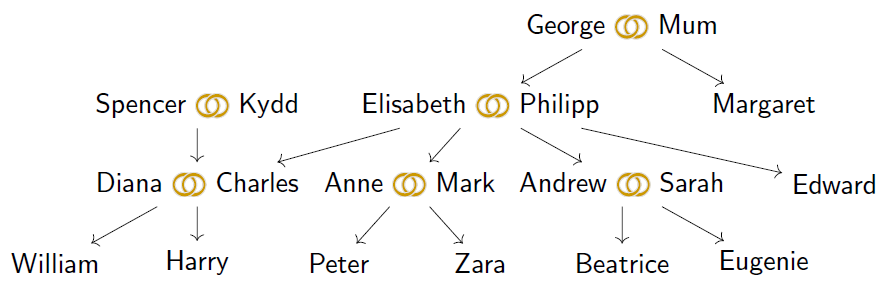
\includegraphics[width=0.5\linewidth]{images/family_tree.png}
\end{figure}
}{ex:family_tree}

\linkterm{Descriptions}{logic_based_inductive_learning} include facts like
\begin{itemize}
    \item $\text{father}(\text{Philip}, \text{Charles})$
    \item $\text{mother}(\text{Mum}, \text{Margaret})$
    \item $\text{married}(\text{Diana}, \text{Charles})$
    \item $\text{male}(\text{Philip})$
    \item $\text{female}(\text{Beatrice})$
\end{itemize}

An analysis of the family tree yields a total of 24 positive instances for the \texttt{grandparent} predicate, categorized by lineage layer:

\begin{itemize}
    \item \textbf{Top-Generation Lineage (George \& Mum)}
    \begin{itemize}
        \item $\text{grandparent}(\text{George}, \text{Charles})$
        \item $\text{grandparent}(\text{George}, \text{Anne})$
        \item $\text{grandparent}(\text{George}, \text{Andrew})$
        \item $\text{grandparent}(\text{George}, \text{Edward})$
        \item $\text{grandparent}(\text{Mum}, \text{Charles})$
        \item $\text{grandparent}(\text{Mum}, \text{Anne})$
        \item $\text{grandparent}(\text{Mum}, \text{Andrew})$
        \item $\text{grandparent}(\text{Mum}, \text{Edward})$
    \end{itemize}

    \item \textbf{Central Royal Lineage (Elisabeth \& Philipp)}
    \begin{itemize}
        \item $\text{grandparent}(\text{Elisabeth}, \text{William})$
        \item $\text{grandparent}(\text{Elisabeth}, \text{Harry})$
        \item $\text{grandparent}(\text{Elisabeth}, \text{Peter})$
        \item $\text{grandparent}(\text{Elisabeth}, \text{Zara})$
        \item $\text{grandparent}(\text{Elisabeth}, \text{Beatrice})$
        \item $\text{grandparent}(\text{Elisabeth}, \text{Eugenie})$
        \item $\text{grandparent}(\text{Philipp}, \text{William})$
        \item $\text{grandparent}(\text{Philipp}, \text{Harry})$
        \item $\text{grandparent}(\text{Philipp}, \text{Peter})$
        \item $\text{grandparent}(\text{Philipp}, \text{Zara})$
        \item $\text{grandparent}(\text{Philipp}, \text{Beatrice})$
        \item $\text{grandparent}(\text{Philipp}, \text{Eugenie})$
    \end{itemize}

    \item \textbf{Maternal Lineage (Spencer \& Kydd)}
    \begin{itemize}
        \item $\text{grandparent}(\text{Spencer}, \text{William})$
        \item $\text{grandparent}(\text{Spencer}, \text{Harry})$
        \item $\text{grandparent}(\text{Kydd}, \text{William})$
        \item $\text{grandparent}(\text{Kydd}, \text{Harry})$
    \end{itemize}
\end{itemize}

\titledbox{Classification Data Split}{
We are currently trying to learn the \texttt{grandparent} rule, so our positive and negative training examples are populated with grandparent facts. For the \texttt{grandparent} relation in this problem instance, the dataset explicitly provides only $12$ positive examples alongside $376$ negative examples:
\begin{itemize}
    \item \textbf{Positive Examples:} e.g., $\text{grandparent}(\text{Mum}, \text{Charles})$
    \item \textbf{Negative Examples:} e.g., $\neg \text{grandparent}(\text{Mum}, \text{Harry})$
\end{itemize}
}

\observationbox{
While there are 24 biological grandparent pairs in the tree, we only need to specify 12 positive examples. The remaining 12 pairs can be completely inferred by the learner by utilizing the \texttt{married} relation present in our background knowledge base ($\mathcal{B}$).
}

\commandnote{
The classification dataset split is derived from the total possible pairwise combinations of individuals in the closed domain under a partial world view:
\begin{itemize}
    \item \textbf{Total Domain Size ($N$):} There are $20$ distinct individuals named in the family tree.
    \item \textbf{Total Relation Space ($N \times N$):} Evaluating every possible candidate pair for the binary predicate $\text{grandparent}(X, Y)$ yields $20 \times 20 = 400$ total possible permutations.
    \item \textbf{Negative Examples Calculation:} Out of the $388$ biologically non-positive pairs ($400 - 24$), we explicitly include $376$ as negative examples. The remaining $12$ true relationships are left completely unlabeled/unclassified to allow the system to infer them via background knowledge (e.g., using the \texttt{married} relation) without causing a logical contradiction.
\end{itemize}
}

\Example{
Without \linkterm{background knowledge}{bg_knowledge}, the system defines \texttt{grandparent} in terms of \texttt{mother} and \texttt{father}:
\[
\text{grandparent(x,y)} \Leftrightarrow (\exists z. \text{mother}(x,z) \land \text{mother}(z,y))
\lor 
(\exists z. \text{mother}(x,z) \land \text{father}(z,y)) \lor \cdots \lor     
(\exists z. \text{father}(x,z) \land \text{father}(z,y)) 
\]
}{}

\commandnote{
Standard \linkterm{attribute}{attribute_based_representations}-based algorithms (like \linkterm{DTs}{decision_trees}) are structurally incapable of learning relational concepts like $\text{grandparent}(X, Y)$.
}

\questionbox{Why?}

Standard machine learning models expect each row in a dataset to represent a single, independent object. To learn a binary relation, the input "object" must be forced into an artificial tuple or pair, such as:
\[
O = \langle \text{Mum}, \text{Charles} \rangle
\]

Because a standard decision tree cannot look up other rows dynamically or link variables across features, we cannot create an abstract column like $\text{parent}(X, Z)$. Instead, we are forced to engineer hyper-specific, hardcoded Boolean attributes for each specific individual in the domain:
\[
\text{FirstElementIsMotherOfElisabeth}(O) \rightarrow \text{True}
\]
\[
\text{SecondElementIsSonOfElisabeth}(O) \rightarrow \text{True}
\]

Lacking the capacity for variables, the induced decision tree cannot uncover the underlying transitivity rule. It simply memorizes the training instances, collapsing into a massive, flat disjunction ($\lor$) of specific lookups:
\[
\text{Grandparent}(O) \Leftrightarrow \left(\text{First}(O) = \text{Mum} \land \text{Second}(O) = \text{Charles}\right) \lor \left(\text{First}(O) = \text{George} \land \text{Second}(O) = \text{Anne}\right) \lor \dots
\]



\titledbox{The Takeaway}{
Attribute-based learning algorithms learn concepts based entirely on the static \defemph{properties of objects}. They are structurally blind to the \defemph{relations between objects}. To effectively learn relational predicates, the hypothesis language must support variables and quantification ($\forall, \exists$), requiring a transition to First-Order Logic via Inductive Logic Programming.
}


\observationbox{
A little bit of \linkterm{background knowledge}{bg_knowledge} helps a lot
}

\Example{
If the \linkterm{background knowledge}{bg_knowledge} contains
\[
\text{parent}(x,y) \Leftrightarrow \text{mother}(x,y) \lor \text{father}(x,y)
\]
Then \texttt{grandparent} can be reduced to:
\[
\text{grandparent}(x,y) \Leftrightarrow (\exists z. \text{parent}(x,z) \land \text{parent}(z,y))
\]
}{}

\anondefinition{
A \defemph{constructive induction} algorithm creates new predicates to facilitate the expression of explanatory \linkterm{hypotheses}{supervised_learning}
}{constructive_induction}

\Example{
Use \linkterm{constructive induction}{constructive_induction} to introduce a predicate \texttt{parent} to simplify the \linkterm{definition}{definitions} of the target \linkterm{predicates}{fol_sig_pl1}
}{}

\titledbox{Bottom-up vs Top-down learning}{
\begin{itemize}
    \item Bottom-up learning: e.g. \linkterm{DTL}{DTL}: start from the observations and work backwards. A \linkterm{DT}{decision_trees} is gradually grown until it is \linkterm{consistent}{consistent_hyp} with the observations
    \item Top-down learning methods start from a general rule and specialize it on every \linkterm{example}{supervised_learning}
\end{itemize}
}

\noindent\makebox[\textwidth]{%
\rule{0.25\textwidth}{0.4pt}\hfill
\textbf{Excursion : Recall - Clauses}\hfill
\rule{0.25\textwidth}{0.4pt}%
}

\anondefinition{
A \textbf{clause} is a disjunction $l_1^{\alpha_1} \lor \cdots \lor l_n^{\alpha_n}$ of \linkterm{literals}{literal}. We use $\square$ for the \textit{"empty"} disjunction (no disjuncts) and call it the \textbf{empty clause}. A clause with exactly one \linkterm{literal}{literal} is called a \textbf{unit clause}.
}{clause_resolution}

\anondefinition{
We often write a \textbf{clause set} $\set{C_1, \cdots, C_n}$ as $C_1 ; \cdots ; C_n$, and write $S ; T$ for the \linkterm{union}{set_union} of the clause sets $S$ and $T$, and $S ; C$ for the extension of $S$ by a \linkterm{clause}{clause_resolution} $C$.
}{clause_set}

\anondefinition{
A \textbf{Horn clause} is a \linkterm{clause}{clause_resolution} with \textbf{at most} one \textbf{positive} \linkterm{literal}{literal}
}{horn_clause}

\titledbox{PROLOG Logic Programming}{
\begin{itemize}
    \item A rule in PROLOG $H:-B_1, \cdots, B_n$ correspond to $H^T \lor B_1^F \cdots B_n^F$, i.e. a \linkterm{Horn clause}{horn_clause}
    \item A goal set (query) $?-G_1, \cdots, G_n$ corresponds to $G_1^F \cdots G_n^F$
    \item A fact $F$ corresponds to the \linkterm{unit clause}{clause_resolution} $F^T$
\end{itemize}
}


\begin{codeblocklst}[caption={PROLOG Example}, label={lst:prolog}]
human(leibniz).
human(sokrates).
greek(sokrates).
fallible(X):-human(X).
\end{codeblocklst}

\Example{
Consider the PROLOG program in \Algref{lst:prolog}

We have three facts, and one rule in the \linkterm{knowledge base}{bg_knowledge}. They translate to the following \linkterm{clause set}{clause_set}:
\begin{enumerate}
    \item $\text{human(leibniz)}^T$
    \item $\text{human(sokrates)}^T$
    \item $\text{greek(sokrates)}^T$
    \item $\text{fallible}(X)^T \lor \text{human}(X)^F$ \hfill ($\text{human}(X) \Rightarrow \text{fallible}(X)$)
\end{enumerate}
}{}

\noindent\makebox[\textwidth]{%
\rule{0.3\textwidth}{0.4pt}\hfill
\textbf{End of Excursion}\hfill
\rule{0.3\textwidth}{0.4pt}%
}

\definition{FOIL}{
\defemph{First-Order Inductive Learner (FOIL)} is a top-down learning algorithm used in \linkterm{ILP}{ILP}. Its main goal is to automatically learn general rules from a \linkterm{set}{def:set} of positive and negative \linkterm{examples}{supervised_learning}, while utilizing existing \linkterm{background knowledge}{bg_knowledge}
}{FOIL}

\ideabox{
\linkterm{FOIL}{FOIL} starts with the most general rule possible and gradually adds \linkterm{literals}{literal} to narrow it down. It continues to make the rule more specific until it perfectly covers positive \linkterm{examples}{supervised_learning} while ruling out the negative ones. 
}


\questionbox{
How would \linkterm{FOIL}{FOIL} learn the \linkterm{predicate}{fol_sig_pl1} \texttt{grandfather} from our family tree from \Exampleref{ex:family_tree}
}

\redbox{
\linkterm{FOIL}{FOIL} constructs a \linkterm{set}{def:set} of \linkterm{Horn clauses}{horn_clause} with head $\text{grandfather}(x,y)$ such that the positive examples are instances of the \texttt{grandfather} relationship
}

We have $12$ total positive examples:
\begin{itemize}
    \item \textbf{Top-Generation Lineage (George \& Mum)}
    \begin{enumerate}
        \item $\text{grandfather}(\text{George}, \text{Charles})$
        \item $\text{grandfather}(\text{George}, \text{Anne})$
        \item $\text{grandfather}(\text{George}, \text{Andrew})$
        \item $\text{grandfather}(\text{George}, \text{Edward})$
    \end{enumerate}

    \item \textbf{Central Royal Lineage (Elisabeth \& Philipp)}
    \begin{enumerate}
        \item $\text{grandfather}(\text{Philipp}, \text{William})$
        \item $\text{grandfather}(\text{Philipp}, \text{Harry})$
        \item $\text{grandfather}(\text{Philipp}, \text{Peter})$
        \item $\text{grandfather}(\text{Philipp}, \text{Zara})$
        \item $\text{grandfather}(\text{Philipp}, \text{Beatrice})$
        \item $\text{grandfather}(\text{Philipp}, \text{Eugenie})$
    \end{enumerate}

    \item \textbf{Maternal Lineage (Spencer \& Kydd)}
    \begin{enumerate}
        \item $\text{grandfather}(\text{Spencer}, \text{William})$
        \item $\text{grandfather}(\text{Spencer}, \text{Harry})$
    \end{enumerate}
\end{itemize}

\textbf{1. Split the Examples}

\begin{itemize}
    \item Positive: e.g. $\tuple{\text{George}, \text{Anne}}, \tuple{\text{Philipp}, \text{Peter}}, \tuple{\text{Spencer}, \text{Harry}}$
    \item Negative: e.g. $\tuple{\text{George}, \text{Elizabeth}}, \tuple{\text{Harry}, \text{Zara}}, \tuple{\text{Charles}, \text{Philipp}}$
\end{itemize}

\textbf{2. Start with the Broadcast Rule}

\linkterm{FOIL}{FOIL} starts with an empty body rule, which basically guesses that everyone is a grandfather to everyone \hfill $\Rightarrow \text{grandfather}(x,y)$. 

In PROLOG, this is equivalent to:

\begin{verbatim}
grandfather(x,y).
\end{verbatim}

or

\begin{verbatim}
grandfather(x,y):-.
\end{verbatim}

This will already include the positive examples but will misclassify all the negative examples.

\textbf{3. Add the "Best" Literal  (Specialization)}

To fix this, \linkterm{FOIL}{FOIL} looks at all possible \linkterm{literals}{literal} it could add to the body of the rule to knock out the negative \linkterm{examples}{supervised_learning}. It tests candidates like:

$\text{father}(x,y) \Rightarrow \text{grandfather}(x,y)$

\begin{verbatim}
grandfather(x,y):-father(x,y)
\end{verbatim}

\redbox{
This incorrectly cuts out 12 positive examples
}

$\text{parent}(x,z) \Rightarrow \text{grandfather}(x,y)$

\begin{verbatim}
grandfather(x,y):-parent(x,z)
\end{verbatim}

\redbox{
This fails to eliminate enough negative examples
}

$\text{father}(x,z) \Rightarrow \text{grandfather}(x,y)$

\begin{verbatim}
grandfather(x,y):-father(x,z)
\end{verbatim}

\observationbox{
This is the only promising candidate, it establishes that $x$ has to be a father to someone $z$
}

\commandnote{
\linkterm{FOIL}{FOIL} uses a \linkterm{heuristic}{heuristic_search} similar to \linkterm{information gain}{information_gain} to mathematically pick the literal that filters out the most negative \linkterm{examples}{supervised_learning} while keeping the positive ones. 
}

\textbf{4. Keep Going}

\linkterm{FOIL}{FOIL} chose the following rule for now $\text{father}(x,z) \Rightarrow \text{grandfather}(x,y)$. There are still some negative \linkterm{examples}{supervised_learning} since being a father doesn't automatically make someone a grandfather. \linkterm{FOIL}{FOIL} repeats the search and appends another \linkterm{literal}{literal} to specialize further. 

Eventually it will find the following rule:

\[
\text{father}(x,z) \land \text{parent}(z,y) \Rightarrow \text{grandfather}(x,y)
\]

\begin{verbatim}
grandfather(x,y):-father(x,z), parent(z,y)
\end{verbatim}

Now, this clause perfectly covers a bunch of positive examples and yields zero negative examples.

\textbf{5. Remove Covered Examples}

\linkterm{FOIL}{FOIL} saves this completed \linkterm{clause}{clause_resolution}
\[
\text{father}(x,z)^F \lor \text{parent}(z,y)^F \lor \text{grandfather}(x,y)^T
\]

It then removes all the positive \linkterm{examples}{supervised_learning} that are successfully explained by this new rule. If there are still unexplained positive \linkterm{examples}{supervised_learning} left, the entire loop starts over to find a second \linkterm{clause}{clause_resolution}

\titledbox{Crucial Constraints}{
Because constructing logical expressions has an incredibly massive branching factor, FOIL enforces strict boundaries to stay efficient:
\begin{itemize}
    \item Variable Connectivity: Any \linkterm{literal}{literal} added must share at least one variable with the variables already present in the \linkterm{clause}{clause_resolution} (either in the head or in a previous \linkterm{literal}{literal}). For example, if trying to define grandfather(x, y), adding married(u, v) is invalid because it introduces completely isolated variables.
    \item Ockham's Razor: To avoid overly complex or "boring" rules, \linkterm{FOIL}{FOIL} limits the length of a \linkterm{clause}{clause_resolution}. If a \linkterm{clause}{clause_resolution} becomes longer than the total number of positive \linkterm{examples}{supervised_learning} it explains, \linkterm{FOIL}{FOIL} flags it as an invalid \linkterm{hypothesis}{supervised_learning} and throws it out.
\end{itemize}
}

\observationbox{
Unlike \linkterm{attribute}{attribute_based_representations}-based learning algorithms that require restructuring data into massive, specific disjunctions (which completely fail to generalize to new family trees), \linkterm{FOIL}{FOIL} outputs clean, highly readable first-order logic rules. Because it can utilize previously learned concepts as \linkterm{background knowledge}{bg_knowledge}, it can master complex structural tasks, e.g. writing correct PROLOG programs for list-processing, from just a handful of examples.
}

\noindent\makebox[\textwidth]{%
\rule{0.25\textwidth}{0.4pt}\hfill
\textbf{Exercise : Inductive Learning}\hfill
\rule{0.25\textwidth}{0.4pt}%
}

Consider the family tree given by the following relations:

\begin{center}
\begin{tabular}{|c|c|} \hline 
    couple & children \\ \hline
    A,B & E,F \\ \hline 
    C,D & G,H \\ \hline 
    F,G & I,J \\ \hline
\end{tabular} 
\end{center}


\begin{figure}[H]
    \centering
    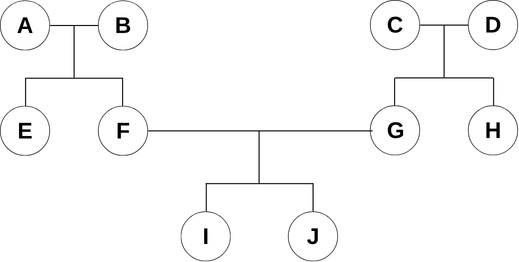
\includegraphics[width=0.5\linewidth]{images/family_tree_ex.png}
\end{figure}

Assume we already know the \linkterm{predicate}{fol_sig_pl1} $\texttt{par}(x,y)$ for $x$ being a parent of $y$. Our goal is to learn the \linkterm{predicate}{fol_sig_pl1} $\texttt{gp}(x,y)$ for $x$ being a grandparent of $y$. That means to find a formula $D$ such that $\forall x,y. \texttt{gp}(x,y) \Leftrightarrow D(x,y)$.

We do not know $D$, but we have the following \linkterm{examples}{supervised_learning} for \texttt{gp}:

\begin{center}
\begin{tabular}{|l|l|}
\hline
person-pair & grandparent \\ \hline
A, I        & yes         \\ 
B, I        & yes         \\ 
A, J        & yes         \\ 
A, E        & no          \\ 
A, F        & no          \\ 
F, A        & no          \\ 
A, A        & no          \\ 
C, J        & yes         \\ 
D, H        & no          \\ 
I, A        & no          \\ \hline
\end{tabular}
\end{center}

\questionbox{
What is the intended formula (call it $D_1$), i.e. the correct definition of grandparent?
}

\answerbox{
$D_1(x,y) = \exists u. \texttt{par}(x,u) \land \texttt{par}(u,y)$
}

\questionbox{
Give a formula $D_2$ that covers exactly the positive \linkterm{examples}{supervised_learning}
}

\answerbox{
\[
D_2(x,y) = (x = A \land y = I) \lor (x = B \land y = I) \lor (x = A \land y = J) \lor (x=C \land y=J) 
\]
}

We want to learn algorithmically the formula 
\[
D(x,y) = \exists u_1, \cdots u_l . L_1 \land \cdots \land L_k
\]

where each $L_i$ is a \linkterm{literal}{literal} of the form 
\[
P(x,y,u_1, \cdots ,u_l)
\]

or 

\[
\neg P(x,y,u_1, \cdots ,u_l)
\]

for some \linkterm{predicate constant}{fol_sig_pl1} $P \in \set{\texttt{par}, \texttt{gp}, =}$

We do so by building the set $\set{L_1, \cdots L_k}$ of \linkterm{literals}{literal} gradually. Each $L_i$ can have free variables in addition to $x$ and $y$, which we will collect at the end as the $u_i$.

\questionbox{
If we start with the empty \linkterm{set}{def:set} of \linkterm{literals}{literal}, give all useful choices that we can make for the first \linkterm{literal}{literal}
}

\answerbox{
If we build the predicate $P$ using only $x$ and $y$, we have the following choices:
\begin{enumerate}
    \item $P(x,y)$
    \item $P(x,x)$
    \item $P(y,x)$
    \item $P(y,y)$
\end{enumerate}

And their negations, so we have total of $8$. 

If we want to introduce a new variable $u$ with the variable connectivity constraint (i.e. at least $x$ or $y$ should be present), we have:
\begin{enumerate}
    \item $P(x,u)$
    \item $P(y,u)$
    \item $P(u,x)$
    \item $P(u,y)$
\end{enumerate}

and their negations, hence another $8$ choices, so we have $16$ choices in total.

Additionally, because $P$ can be the equality relation, we have:
\begin{enumerate}
    \item $x = y$
    \item $x \neq y$
\end{enumerate}

Note that it is useless to add equality checks with a new variable or where both variables are the same.

So we have $16$ choices for $P \in \set{\texttt{par}, \texttt{gp}}$ and $2$ choices for $P \in \set{=}$
}

\questionbox{
For each choice $L$ that is:
\begin{itemize}
    \item non-recursive (i.e. $P$ is not the target predicate $\texttt{gp}$), 
    \item positive (i.e. the \linkterm{literal}{literal} is not negated),
    \item not an equality (i.e. $P \notin \set{=}$), and
    \item does not introduce a new variable (i.e. only $x$ and $y$) 
\end{itemize}
Which \linkterm{examples}{supervised_learning} are falsely classified?
}


Now we are limited to these four choices:
\begin{enumerate}
    \item $\texttt{par}(x,x)$
    \item $\texttt{par}(y,y)$
    \item $\texttt{par}(x,y)$
    \item $\texttt{par}(y,x)$
\end{enumerate}

Let's analyze each of these \linkterm{literals}{literal} to see which \linkterm{examples}{supervised_learning} they falsely classify:

$\texttt{par}(x,x)$:

i.e. we are saying that $\texttt{par}(x,x) \Rightarrow \texttt{gp}(x,y)$

i.e. we are asserting in, e.g. PROLOG \inlinecode{gp(x,y) :- par(x,x)}. Meaning, $x$ is grandparent of $y$ if $x$ is parent of $x$. 

Obviously, there are no \linkterm{examples}{supervised_learning} where this holds, hence it will be false for all \linkterm{examples}{supervised_learning}.

It will not give true at all $\leadsto$ no false positives. It will always give false $\leadsto$ we will have $6$ true negatives and $4$ false negatives.

\observationbox{
We have a similar situation for $\texttt{par}(y,y)$ (4 falsely classified \linkterm{examples}{supervised_learning})
}

$\texttt{par}(x,y)$:

i.e. we are saying that $\texttt{par}(x,y) \Rightarrow \texttt{gp}(x,y)$

i.e. we are asserting in, e.g. PROLOG \inlinecode{gp(x,y) :- par(x,y)}. Meaning, $x$ is grandparent of $y$ if $x$ is parent of $y$. 

We will have $4$ false negatives (for the actual grandparents in the data)

For the six negative \linkterm{examples}{supervised_learning}, we have $\tuple{A,E}$, $\tuple{A,F}$, $\tuple{D,H}$ where $\texttt{par}(x,y)$ holds, this yields $3$ false positives.

\observationbox{
This has a higher number of falsely classified \linkterm{examples}{supervised_learning} ($7$)
}

$\texttt{par}(y,x)$:

i.e. we are saying that $\texttt{par}(y,x) \Rightarrow \texttt{gp}(x,y)$

i.e. we are asserting in, e.g. PROLOG \inlinecode{gp(x,y) :- par(y,x)}. Meaning, $x$ is grandparent of $y$ if $y$ is parent of $x$. 

Again this will misclassify the actual positives we have $\leadsto 4$ false negatives. 

For the negative \linkterm{examples}{supervised_learning}, $\texttt{par}(y,x)$ will hold for $\tuple{F,A}$, hence we have $1$ false positive.

\observationbox{
This \linkterm{literal}{literal} misclassify $5$ \linkterm{examples}{supervised_learning}
}

\commandnote{
There were no true positives for all the 4 choices. The positive examples were always false negatives.
}

\noindent\makebox[\textwidth]{%
\rule{0.3\textwidth}{0.4pt}\hfill
\textbf{End of Exercise}\hfill
\rule{0.3\textwidth}{0.4pt}%
}